\section{طراحی و شبیه‌سازی کنترل‌کننده برای کانال رول}\label{roll_lqr_section_simulation}
در بخش
\ref{quadall3}
شبیه‌سازی استند سه درجه آزادی چهارپره انجام شد.
در این بخش به کنترل زاویه رول با فرض مقید‌بودن زاویه پیچ و یاو پرداخته خواهد شد. به این منظور، در بخش نتایج شبیه‌سازی برای تعقیب مقدار مطلوب خروجی زاویه رول ارائه می‌شود. سپس، در بخش عملکرد کنترل‌کننده در  حضور نویز اندازه‌گیری بررسی می‌شود.
\subsection{تعقیب مقدار مطلوب خروجی}


 در این بخش به بررسی عملکرد چهارپره در حضور کنترل‌کننده \lr{LQR} پرداخته می‌شود. در شبیه‌سازی برای بهینه‌سازی ضرایب وزنی \lr{LQR} از روش بهینه‌سازی
\lr{TCACS} \cite{Karimi2010}
استفاده شده‌است.
\begin{figure}[H]
	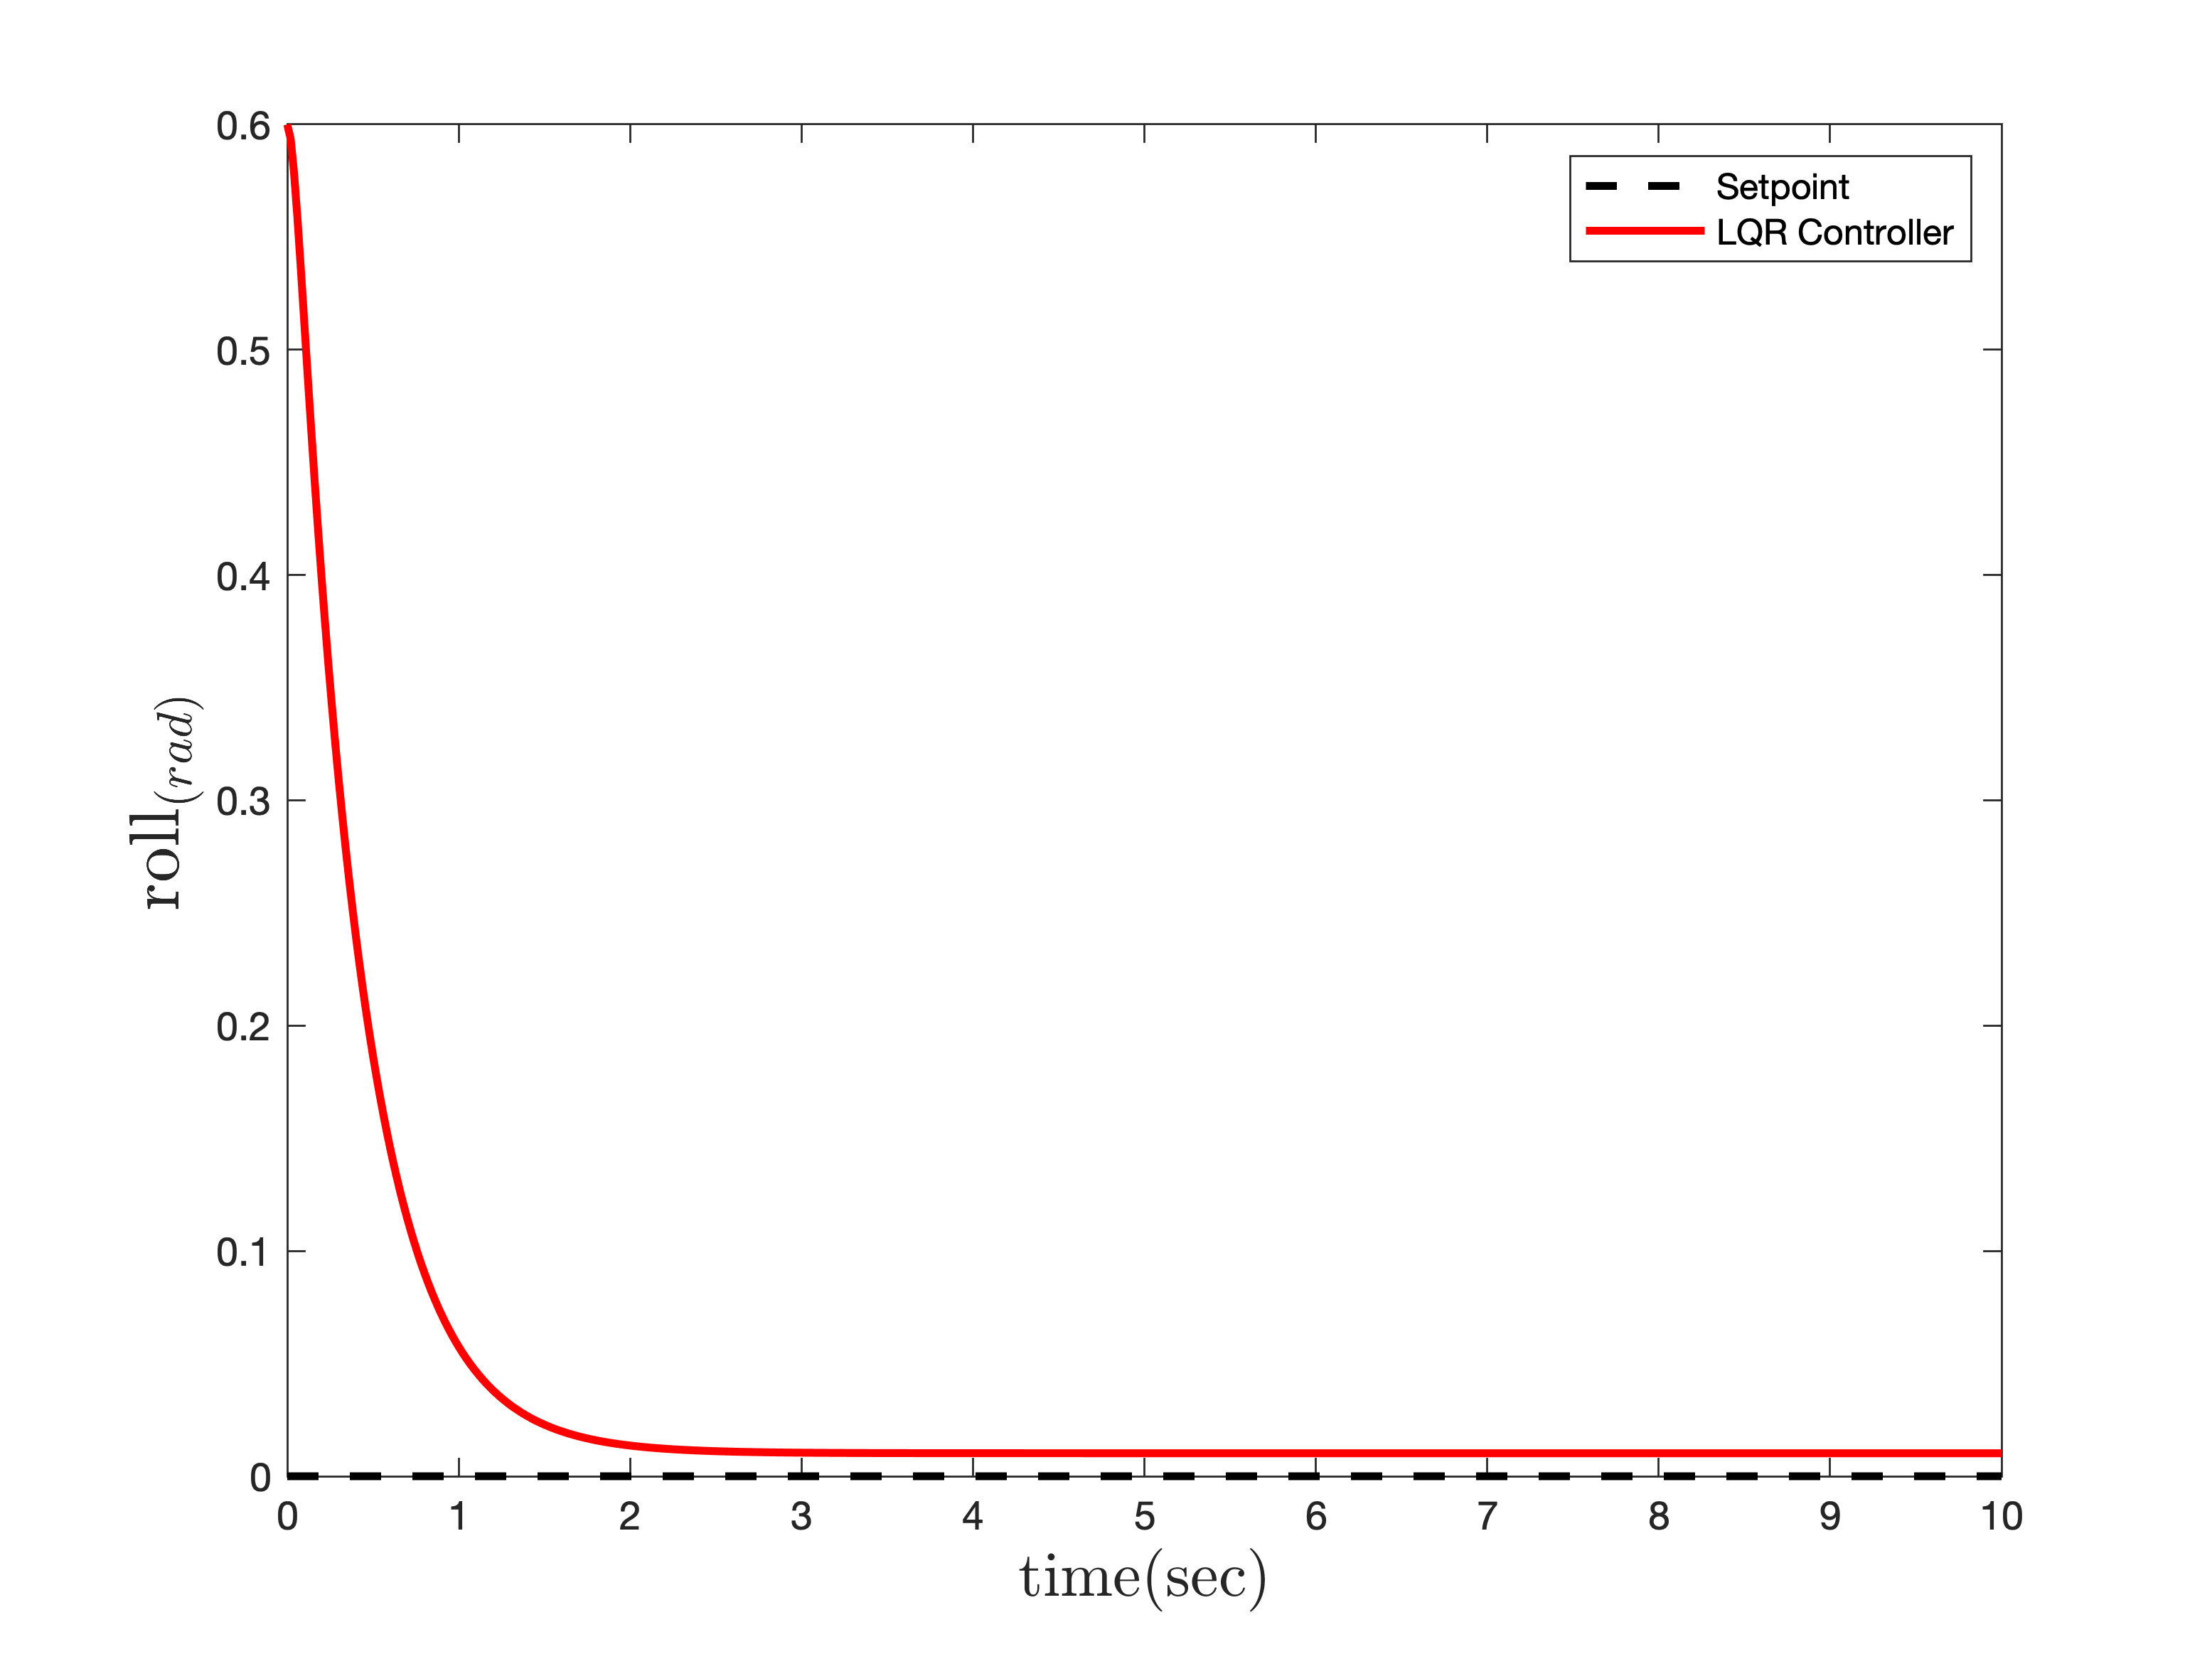
\includegraphics[width=.48\linewidth]{../Figures/MIL/LQR/Roll/lqr_roll_nn.png}
	\centering
	\caption{عملكرد \lr{LQR} در کنترل زاويه رول (تعقیب ورودی صفر)}
	\label{lqr_roll_figure_simulation}
\end{figure}
\begin{figure}[H]
	\centering
	\subfigure[موتور شماره دو]{
		\centering
		\includegraphics[width=.45\linewidth]{../Figures/MIL/LQR/Roll/lqr_roll_Omega_2_nn.png}
	}
	\subfigure[موتور شماره چهار]{
		\centering
		\includegraphics[width=.45\linewidth]{../Figures/MIL/LQR/Roll/lqr_roll_Omega_4_nn.png}
	}
	\caption{‫‪فرمان کنترلی موتورها در کنترل زاویه رول (تعقیب ورودی صفر)}
\end{figure}


بر اساس خروجی شبیه‌سازی (شکل
\ref{lqr_roll_figure_simulation})،
کانال رول در حضور کنترل‌کننده \lr{LQR} در حدود پنج ثانیه به تعادل می‌رسد اما دارای خطای ماندگار است. 